% !TEX root = main_min_disc_dist.tex


\begin{IEEEbiography}[{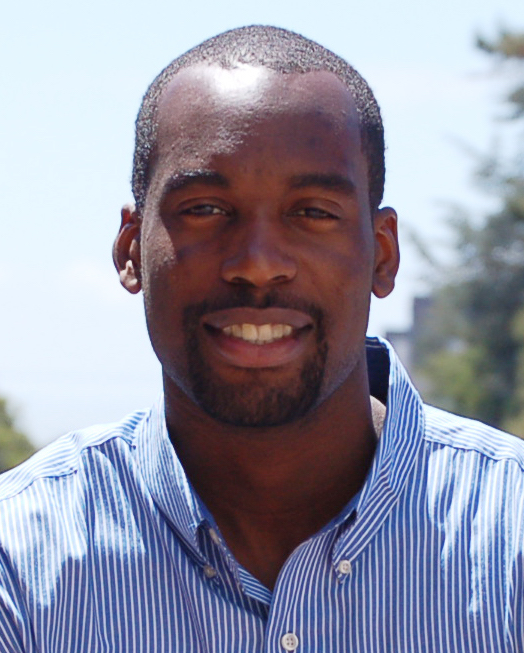
\includegraphics[width=1in,height=1.25in,clip,keepaspectratio]{bio/kene}}]{Anayo K. Akametalu} is a PhD. candidate in Electrical Engineering and Computer Sciences at the University of California, Berkeley. He obtained his B.S. degree in Electrical Engineering from the University of California, Santa Barbara in 2012. His research interests lie at the intersection of control theory and reinforcement learning. He has been funded through the National Science Foundation Bridge to Doctorate Fellowship, UC Berkeley Chancellor's Fellowship, and GEM Fellowship.\end{IEEEbiography}
\vspace{-6cm}
\begin{IEEEbiography}[{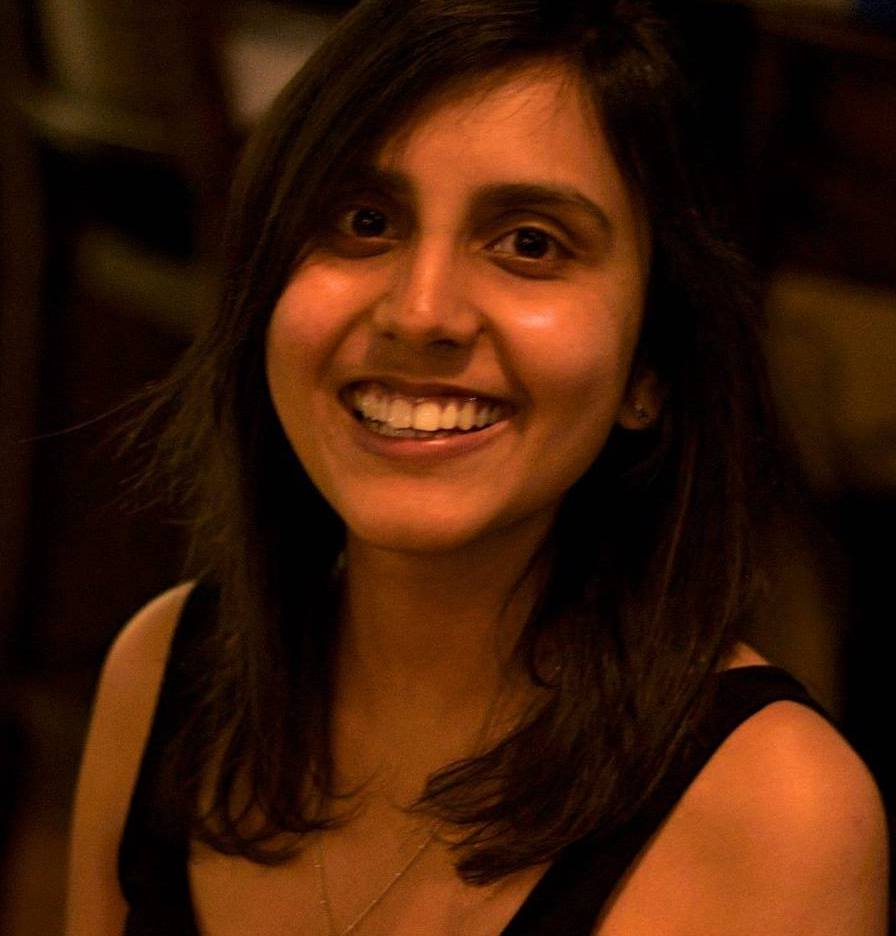
\includegraphics[width=1in,height=1.25in,clip]{bio/shromona}}]{Shromona Ghosh} received her Bachelor in Technology in Electronics and Communication Engineering from National Institute of Technology, Karnataka in 2013. She is currently a PhD candidate at University of California, Berkeley . Her research interests lie in the intersection of Formal Methods, Control Theory and Machine Learning. Specifically, she is looking into developing tools for the formal analysis of systems with learning components. 
\end{IEEEbiography}
\vspace{-6cm}
\begin{IEEEbiography}[{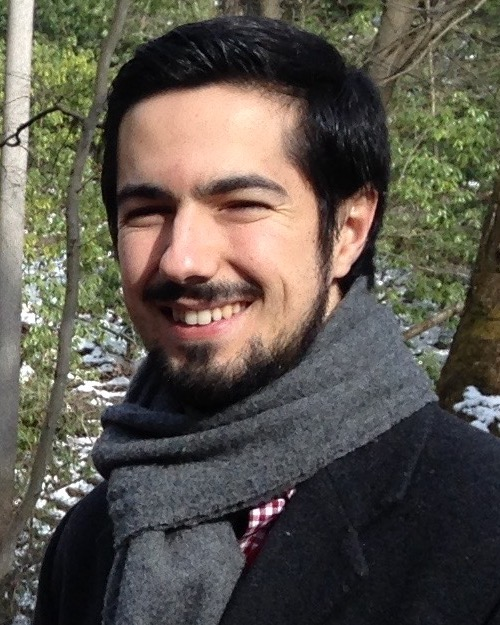
\includegraphics[width=1in,height=1.25in,clip,keepaspectratio]{bio/jaime}}]{Jaime F. Fisac} is a Ph.D. candidate in Electrical Engineering and Computer Sciences at the University of California, Berkeley. He received a B.S./M.S. degree in Electrical Engineering from the Universidad Polit{\'e}cnica de Madrid, Spain, in 2012, and a M.Sc. in Autonomous Vehicle Dynamics and Control from Cranfield University, UK, in 2013. He is a recipient of the ``la~Caixa'' Foundation Fellowship (2013-2015). His research interests lie in control theory, artificial intelligence, and cognitive science, with a focus on safety for robotic and AI systems operating closely with people.
\end{IEEEbiography}
\vspace{-6cm}
\begin{IEEEbiography}[{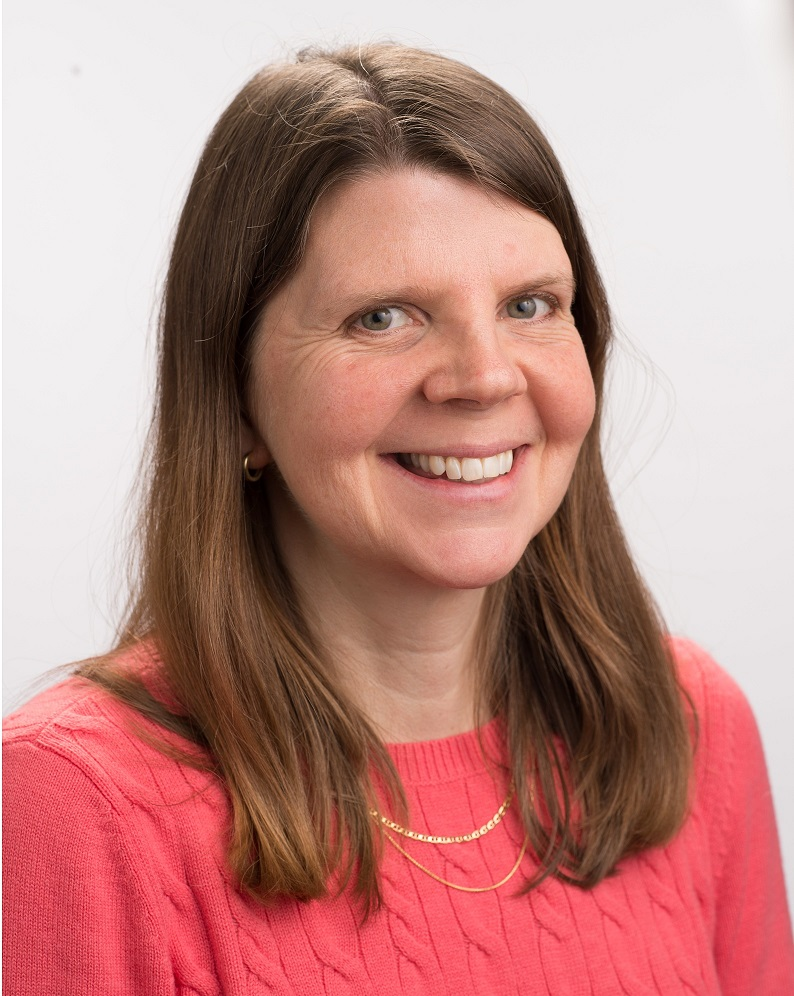
\includegraphics[width=1in,height=1.25in,clip,keepaspectratio]{bio/claire}}]{Claire J. Tomlin} is the Charles A. Desoer Professor of Engineering in Electrical Engineering and Computer Sciences at the University of California, Berkeley. She was an Assistant, Associate, and Full Professor in Aeronautics and Astronautics at Stanford from 1998 to 2007, and in 2005 joined Berkeley. Claire works in the area of control theory and hybrid systems, with applications to air traffic management, UAV systems, energy, robotics, and systems biology. She is a MacArthur Foundation Fellow (2006) and an IEEE Fellow (2010), and in 2010 held the Tage Erlander Professorship of the Swedish Research Council at KTH in Stockholm.
\end{IEEEbiography}